\documentclass[border=6pt]{standalone}
\usepackage[T1]{fontenc}
\usepackage{lmodern}
\usepackage{tikz}
\usetikzlibrary{positioning, arrows.meta, calc, fit, backgrounds, shapes.geometric}

\definecolor{ibmblue}{HTML}{0F62FE}
\definecolor{ibmred}{HTML}{DA1E28}
\definecolor{graymute}{HTML}{A8A8A8}
\definecolor{graydark}{HTML}{6F6F6F}
\definecolor{graylight}{HTML}{F4F4F4}
\definecolor{inkblack}{HTML}{161616}

\begin{document}
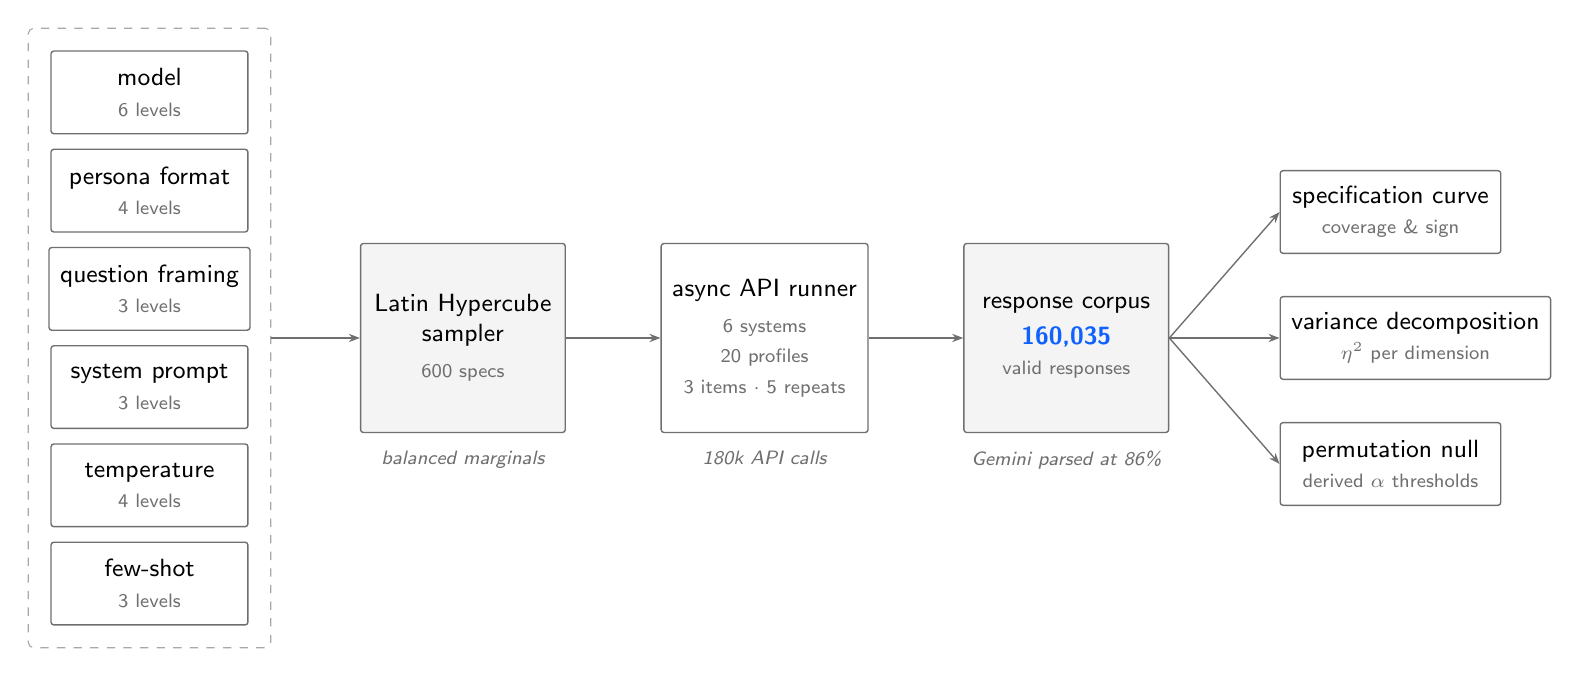
\begin{tikzpicture}[
    font=\sffamily\small,
    every node/.style={align=center},
    stage/.style={
        draw=graydark, line width=0.5pt, fill=white,
        minimum width=2.5cm, minimum height=1.05cm, rounded corners=1pt,
        inner sep=4pt, font=\sffamily\small
    },
    group/.style={
        draw=graymute, dashed, line width=0.4pt, rounded corners=2pt,
        inner sep=8pt
    },
    arrow/.style={
        -{Stealth[length=4pt, width=3pt]},
        line width=0.5pt, draw=graydark
    },
    label/.style={font=\sffamily\scriptsize\itshape, text=graydark},
    grouplabel/.style={font=\sffamily\scriptsize\bfseries, text=inkblack}
]

\node[stage] (model)   {model\\\textcolor{graydark}{\scriptsize 6 levels}};
\node[stage, below=0.18cm of model] (persona) {persona format\\\textcolor{graydark}{\scriptsize 4 levels}};
\node[stage, below=0.18cm of persona] (framing) {question framing\\\textcolor{graydark}{\scriptsize 3 levels}};
\node[stage, below=0.18cm of framing] (sysp)    {system prompt\\\textcolor{graydark}{\scriptsize 3 levels}};
\node[stage, below=0.18cm of sysp]    (temp)    {temperature\\\textcolor{graydark}{\scriptsize 4 levels}};
\node[stage, below=0.18cm of temp]    (fewshot) {few-shot\\\textcolor{graydark}{\scriptsize 3 levels}};

\begin{scope}[on background layer]
    \node[group, fit=(model)(fewshot), label={[grouplabel, anchor=south]north:Prompt dimensions $\cdot$ 2{,}592 cells}] (dims) {};
\end{scope}

\node[stage, right=1.4cm of $(framing.east)!0.5!(sysp.east)$, minimum height=2.4cm, minimum width=2.6cm,
      fill=graylight] (lhs) {Latin Hypercube\\sampler\\[2pt]\textcolor{graydark}{\scriptsize 600 specs}};

\node[stage, right=1.2cm of lhs, minimum height=2.4cm, minimum width=2.6cm] (runner)
     {async API runner\\[2pt]\textcolor{graydark}{\scriptsize 6 systems}\\\textcolor{graydark}{\scriptsize 20 profiles}\\\textcolor{graydark}{\scriptsize 3 items $\cdot$ 5 repeats}};

\node[stage, right=1.2cm of runner, minimum height=2.4cm, minimum width=2.6cm,
      fill=graylight] (data) {response corpus\\[2pt]\textcolor{ibmblue}{\bfseries 160{,}035}\\\textcolor{graydark}{\scriptsize valid responses}};

\node[stage, right=1.4cm of data, yshift=1.6cm, minimum width=2.8cm] (curve)
     {specification curve\\\textcolor{graydark}{\scriptsize coverage \& sign}};
\node[stage, right=1.4cm of data, minimum width=2.8cm] (eta)
     {variance decomposition\\\textcolor{graydark}{\scriptsize $\eta^2$ per dimension}};
\node[stage, right=1.4cm of data, yshift=-1.6cm, minimum width=2.8cm] (perm)
     {permutation null\\\textcolor{graydark}{\scriptsize derived $\alpha$ thresholds}};

\draw[arrow] (dims.east) -- (lhs.west);
\draw[arrow] (lhs.east)  -- (runner.west);
\draw[arrow] (runner.east) -- (data.west);
\draw[arrow] (data.east) -- (curve.west);
\draw[arrow] (data.east) -- (eta.west);
\draw[arrow] (data.east) -- (perm.west);

\node[label, below=0.10cm of lhs] {balanced marginals};
\node[label, below=0.10cm of runner] {180k API calls};
\node[label, below=0.10cm of data]   {Gemini parsed at 86\%};

\end{tikzpicture}
\end{document}
